\documentclass[9pt,twocolumn,twoside,lineno]{gsag3jnl}

\articletype{gs} % Genomic Selection

% Theorem-like environments for the propositions and their proofs.
\usepackage{amsthm}
\theoremstyle{plain}
\newtheorem{proposition}{Proposition}
\theoremstyle{remark}
\newtheorem{remark}{Remark}

% Numeric placeholder macro carried over from the single-column source.
\newcommand{\NUM}[1]{#1}

\title{Metric-consistent neural networks for genomic prediction and selection: a standardized-MSE Pearson loss, affine calibration, and selection-aware evaluation}

\author[$\ast$,$\dagger$,1]{Gr\'egory Beurier}
\author[$\ast$,$\dagger$]{Denis Cornet}
\author[$\ast$,$\dagger$]{Lauriane Rouan}
\author[$\ast$,$\dagger$]{David Cros}

\affil[$\ast$]{CIRAD, UMR AGAP Institut, Montpellier, France}
\affil[$\dagger$]{UMR AGAP Institut, Univ Montpellier, CIRAD, INRAE, Institut Agro, Montpellier, France}

\keywords{genomic prediction \\ genomic selection \\ deep learning \\ loss functions \\ calibration}

\runningtitle{Metric-consistent neural networks for genomic prediction}

\runningauthor{Beurier \textit{et al.}}

\begin{abstract}
Genomic prediction models are trained almost universally to minimize the mean squared error (MSE), yet they are evaluated, and used for selection, by the Pearson correlation $r$ between predicted and observed phenotypes and by genotype ranking. That maximizing $r$ equals minimizing the MSE of standardized variables, $\mathrm{MSE}(z_y,z_{\hat y})=2(1-r)$, is elementary, and correlation, concordance (CCC) and ranking losses have been used before; our contribution is a systematic, calibration- and selection-metric-aware empirical characterization of these losses across 101 trait--dataset combinations from 12 panels/sources spanning 10 species (EasyGeSe, CIMMYT wheat, SoyNAM), with a closed-form affine recalibration. We use it only as a stable training target; one affine map restores scale and offset, leaving $r$ and all rankings unchanged whenever the validation-fitted map is increasing, which holds in $>99\%$ of folds ($r$-sign flips in only $0.91\%$). Holding architecture, splits and tuning fixed so that only the loss differs, and comparing each architecture against its own MSE baseline, correlation and CCC losses raised predictive ability (cell-level $\Delta r$ from $+0.038$ to $+0.044$; Holm-corrected paired Wilcoxon $p<10^{-7}$, corroborated by a mixed model whose confidence intervals exclude zero) and selection metrics (NDCG@10 $+0.016$; relative efficiency $+0.04$). The benefit is strongly architecture-dependent --- large for the Transformer and CNN, negligible for the MLP. Only CCC lowered pooled calibrated RMSE in the per-cell bootstrap (not corroborated by the mixed model). No neural loss unseated the GBLUP or ridge baselines on mean rank. Correlation-consistent training is thus a useful, well-characterized tool, not a universal replacement for MSE.
\end{abstract}

\begin{document}

\maketitle
\thispagestyle{firststyle}
\logomark
\articletypemark
\marginmark
\firstpagefootnote

\correspondingauthoraffiliation{1}{Corresponding author: CIRAD, UMR AGAP Institut, Montpellier, France. E-mail: gregory.beurier@cirad.fr}
\vspace{-34pt}% Only used for adjusting extra space in the left column of the first page

\section{Introduction}

Genomic selection \citep{meuwissen2001} predicts the genetic merit of candidate
individuals from genome-wide markers, and has become central to modern plant and
animal breeding \citep{heffner2009,jannink2010,desta2014}. The dominant
parametric baseline, genomic best linear unbiased prediction
(GBLUP)/ridge-regression BLUP \citep{vanraden2008,endelman2011}, is increasingly
complemented by machine-learning and deep-learning predictors
\citep{ma2018deepgs,wang2023dnngp,montesinos2021review,montesinos2021power}.
Whether deep learning improves on GBLUP remains dataset-dependent: recent
comparisons find that neither systematically dominates, and that outcomes hinge
on tuning, architecture and the choice of evaluation metric
\citep{montesinos2025dlgblup}.

That last point is the subject of this paper. Genomic predictors are trained, by
near-universal default, to minimize the mean squared error (MSE). But they are
\emph{assessed} with the Pearson correlation $r$ between predicted and observed
phenotypes --- the ``predictive ability'' reported in essentially every genomic
prediction study \citep{crossa2010} --- and they are \emph{used} to rank
candidates and select the best ones. There is therefore a systematic mismatch
between the training objective and the objective that actually matters.
\citet{waldmann2019} showed that selecting a model by $r$ can disagree with
selecting it by MSE or $R^2$. \citet{ornella2014} argued that $r$ is a poor guide
to performance in the tails of the distribution, where selection actually
operates, and evaluated the recovery of the best $\alpha\in\{10,\dots,40\}\%$ of
individuals. \citet{blondel2015} reframed genomic selection as a ranking problem,
introduced NDCG from information retrieval as an accuracy measure, and reported
that $r$ correlates poorly with ranking quality.

If correlation is the target, why not train for it directly? A recent
convolutional architecture for genomic selection states plainly that ``Pearson
correlation cannot be set as the loss function'' and substitutes a family of
$L_p$ losses \citep{pnngs2024}. We show this premise is false. The Pearson
correlation \emph{is} a loss --- a standardized MSE --- and training with it is
both well posed and numerically stable. The remaining objection to a correlation
loss, that it ignores scale and offset, is real but easily and provably remedied
by an affine recalibration applied after training.

\subsubsection{Contributions:}
\begin{enumerate}
\item \textbf{A standardized-MSE Pearson loss (Section~\nameref{sec:prop1}).} We give
the exact identity $\mathrm{MSE}(z_y,z_{\hat y}) = 2(1-r)$ and use it as a stable,
differentiable training objective, verified numerically (to single-precision
tolerance for the loss; to float64 machine precision for the calibration identity).
\item \textbf{Affine calibration with a closed form
(Section~\nameref{sec:prop2}).} We prove that the optimal post-hoc affine map yields
residual error $\sigma_y^2(1-r^2)$ and restores scale and offset while preserving
$r$ and all rankings --- turning the scale-invariance ``weakness'' of correlation
into a controlled, two-parameter calibration step.
\item \textbf{Mini-batch analysis (Section~\nameref{sec:prop3}).} We show the
mini-batch Pearson loss is a biased surrogate for the global objective and
quantify the effect of batch size empirically.
\item \textbf{A reproducible, selection-aware benchmark
(Sections~\nameref{sec:methods}--\nameref{sec:results}).} Across 101
trait--datasets from 12 panels/sources spanning 10 species, with architecture, splits and tuning held
fixed so that only the loss changes, we report both predictive and
selection-oriented metrics, a confirmatory mixed-model analysis, and a
meta-analysis of \emph{when} correlation-consistent training helps. All data are
public and all code, splits and tuned configurations are released.
\end{enumerate}

\noindent We do not claim that a Pearson loss is uniformly superior to MSE; that
would be false. We provide a principled, reproducible framework for training,
calibrating and evaluating neural genomic predictors when the breeding objective
is correlation and ranking rather than raw squared error.

\section{Theory}\label{sec:theory}
Throughout, $y,\hat y\in\mathbb{R}^n$, with sample means $\bar y,\bar{\hat y}$ and
population variances $\sigma_x^2 = \tfrac1n\sum_i (x_i-\bar x)^2$. The Pearson
correlation is $r=r(y,\hat y)=\tfrac1n\sum_i z_{y,i} z_{\hat y,i}$ where
$z_{x,i}=(x_i-\bar x)/\sigma_x$ is the standardized variable.

\subsection{The Pearson loss is a standardized MSE}\label{sec:prop1}
\begin{proposition}\label{prop:1}
For non-degenerate $y,\hat y$ (i.e.\ $\sigma_y,\sigma_{\hat y}>0$),
\[
\mathrm{MSE}(z_y,z_{\hat y}) \;=\; \tfrac1n\sum_{i=1}^n (z_{y,i}-z_{\hat y,i})^2
\;=\; 2\,(1-r).
\]
Consequently $1-r = \tfrac12\,\mathrm{MSE}(z_y,z_{\hat y})$, and minimizing the
standardized MSE is exactly maximizing the Pearson correlation.
\end{proposition}
\begin{proof}
Expanding the square,
$\tfrac1n\sum_i (z_{y,i}-z_{\hat y,i})^2
= \tfrac1n\sum_i z_{y,i}^2 - 2\tfrac1n\sum_i z_{y,i} z_{\hat y,i}
+ \tfrac1n\sum_i z_{\hat y,i}^2 = 1 - 2r + 1 = 2(1-r)$,
because $\tfrac1n\sum_i z_{x,i}^2 = 1$ by construction and
$\tfrac1n\sum_i z_{y,i} z_{\hat y,i}=r$.
\end{proof}
This gives the loss $\mathcal{L}_{\mathrm{P}}(\hat y,y) = 1-r(\hat y,y)$,
implemented as $\tfrac12\,\mathrm{MSE}(z_y,z_{\hat y})$ with a small $\varepsilon$
guarding the standardization denominators. It is differentiable everywhere
$\sigma_{\hat y}>0$; we verify the gradient against finite differences and verify
the identity to single-precision tolerance in Section~\nameref{sec:res-numerical}. The
negative-correlation loss $-r$ differs from $\mathcal{L}_{\mathrm{P}}$ by a
constant and has identical gradients.

\subsection{Affine calibration restores scale without changing rank}\label{sec:prop2}
Correlation is invariant to strictly increasing affine transformations of $\hat
y$: a model trained on $\mathcal{L}_{\mathrm{P}}$ controls the \emph{shape} of the
prediction but not its scale or offset. This is corrected exactly and cheaply.
\begin{proposition}\label{prop:2}
Let $p\in\mathbb{R}^n$ be raw predictions and $r=r(y,p)$. The affine map
$\tilde y = a\,p+b$ minimizing $\tfrac1n\sum_i (a p_i + b - y_i)^2$ has
\[
a^\star = \frac{\mathrm{cov}(y,p)}{\mathrm{var}(p)},\qquad
b^\star = \bar y - a^\star\,\bar p,\qquad
\mathrm{MSE}_{\min} = \sigma_y^2\,(1-r^2).
\]
If $a^\star>0$, the map is strictly increasing and hence preserves $r$, the
Spearman correlation, and every top-$k$/ranking quantity, while setting the
calibration slope to $1$ and intercept to $0$.
\end{proposition}
\begin{proof}
Ordinary least squares for a single predictor gives $a^\star,b^\star$ as stated;
the minimized residual variance of simple linear regression is
$\sigma_y^2(1-r^2)$. A strictly increasing transform preserves the order of $p$
and leaves correlation-type and rank-based statistics unchanged.
\end{proof}
We fit $(a^\star,b^\star)$ on held-out validation predictions (never on the test
set) and apply them to the test predictions. Isotonic regression provides a
monotone non-linear alternative when the raw-vs-true relationship is monotone but
curved. Calibration cannot change $r$ but can dramatically improve RMSE, bias and
the calibration slope (Figure~\ref{fig:simulation}; Section~\nameref{sec:res-calibration}).

\subsection{Mini-batch versus global Pearson}\label{sec:prop3}
\begin{proposition}\label{prop:3}
For a partition of the data into batches $B_1,\dots,B_K$, the batch-averaged loss
$\tfrac1K\sum_k \bigl(1-r_{B_k}\bigr)$ is not equal to $1-r_{\mathrm{global}}$ in
general, because $r$ is a non-linear (ratio-of-moments) functional of the data.
The discrepancy and the variance of the gradient estimate grow as the batch size
decreases.
\end{proposition}
A full-batch (or large-batch) evaluation of $\mathcal{L}_{\mathrm{P}}$ therefore
optimizes the global objective, whereas small batches optimize a noisier
surrogate. We quantify the practical consequence for training stability and
predictive ability in Section~\nameref{sec:res-batch}.

\subsection{Multi-trait and group-aware variants}\label{sec:groupaware}
The loss extends naturally to $T$ traits, $\mathcal{L}=\tfrac1T\sum_{t=1}^T
(1-r_t)$ (or a weighted sum $\sum_t w_t(1-r_t)$), and to a group-aware objective
$\mathcal{L}=\tfrac1G\sum_{g=1}^G (1-r_g)$ where $g$ indexes environments, years,
families or sites --- aligning training with the within-environment correlation
that multi-environment breeding programs actually care about. As in
Proposition~\ref{prop:3}, neither variant equals the pooled global correlation.

\section{Materials and Methods}\label{sec:methods}

\subsection{Datasets}
We use three public sources, for a total of 101
trait--dataset combinations across 12 panels/sources spanning 10 species. (i) \emph{EasyGeSe}
\citep{quesada2025easygese}: a benchmark of ten species (barley, common bean,
lentil, maize, eastern oyster, pig, loblolly pine, rice, soybean and wheat)
providing genotypes, phenotypes and \emph{fixed} cross-validation partitions; the
maize set is the global genotype-by-environment competition panel
\citep{washburn2025maize}. (ii) The CIMMYT \emph{wheat} panel
\citep{crossa2010}: 599 lines, 1{,}279 DArT markers and grain yield in four
environments, used for cross-environment transfer. (iii) \emph{SoyNAM}
\citep{xavier2016soynam}: $\sim$5{,}500 recombinant inbred lines in 40 biparental
families, used for leave-family-out prediction. Genotypes are coded as allele
dosages; preprocessing (unsupervised, no phenotype) applies a minor-allele
frequency filter ($\geq 0.01$), mean imputation, and a top-variance cap at
20{,}000 markers for the seven panels whose marker count exceeded 20{,}000
(barley, lentil, maize, oyster, pig, rice and soybean).
Table~\ref{tab:datasets} and Figure~\ref{fig:datasets} summarize the data.

\subsection{Models}
The parametric baseline is GBLUP with REML-estimated variance
components, implemented in the spectral basis of the linear genomic kernel
$K=XX^\top/p$ and validated against the \texttt{rrBLUP} package
\citep{endelman2011} to floating-point precision (cross-implementation
correlation $1.0000$). We also include ridge regression as a linear baseline. The neural predictors
are a multilayer perceptron (MLP), a one-dimensional convolutional network over
ordered markers (1D-CNN), and a light Transformer over marker patches. Crucially,
\emph{the architecture is held fixed across losses}: it is tuned once per
(dataset, model) with a neutral MSE objective and then frozen, so that the only
thing that changes in the loss comparison is the loss.

\subsection{Loss functions}
We compare MSE; the standardized-MSE Pearson loss
$1-r$ (Proposition~\ref{prop:1}); a hybrid $\,(1-r)+\lambda\,\mathrm{MSE}\,$ with
$\lambda=0.1$; and a concordance-correlation loss $1-\rho_c$ \citep{lin1989},
which penalizes correlation, scale and offset jointly. The negative-Pearson and
explicit standardized-MSE forms are included in the numerical checks.

\subsection{Calibration}
For every model and loss we report predictions under
three post-hoc maps: raw (identity), affine (Proposition~\ref{prop:2}) and
isotonic. Calibrators are fit on validation predictions only.

\subsection{Cross-validation}
We use the fixed EasyGeSe partitions (5 folds
$\times$ 2 repeats $=$ 10 folds per trait), repeated $K$-fold for wheat and SoyNAM, leave-family-out for
SoyNAM, and cross-environment transfer for wheat. Within each training fold an
inner 80/20 split (group-aware for family CV) provides early-stopping and
calibration data; markers are standardized with training statistics only;
targets are standardized with training statistics for the neural networks and
predictions are returned in the original units. Neural networks early-stop on the
validation value of the loss being trained. The test fold is never used for
fitting, early stopping, calibration or hyper-parameter selection.

\subsection{Evaluation metrics}
Predictive: Pearson $r$, Spearman $\rho$, RMSE,
MAE, $R^2$, mean bias, and the calibration slope and intercept (ideal $1$ and
$0$). Selection-aware, at intensities $k\in\{5,10,15,20\}\%$: top-$k$ overlap,
precision@$k$, recall@$k$, NDCG@$k$ \citep{jarvelin2002ndcg}, selection
differential, mean phenotype of the selected, and relative efficiency (achieved
gain divided by the oracle gain).

\subsection{Statistical Analysis}
For each cell we average over folds and form
$\Delta m = m_{\mathrm{loss}}-m_{\mathrm{MSE}}$ within the same architecture.
We report bootstrap confidence intervals (bias-corrected and accelerated, BCa,
when $n\geq12$; the percentile bootstrap otherwise, as for the $n=4$ split and
$n=8$ sorghum contrasts), paired Wilcoxon tests with
Holm and Benjamini--Hochberg \citep{benjamini1995} correction, and mean method
ranks. As a corroborative analysis we fit a linear mixed model
\citep{bates2015lme4} on cell-level means (one observation per
dataset$\times$trait$\times$model$\times$loss, which avoids fold-level
pseudoreplication), $\textit{metric}\sim \textit{loss}+\textit{model}+(1\mid
\textit{dataset})+(1\mid \textit{dataset:trait})$ with MSE as the reference level.
The primary inference is the cell-level paired contrast; the mixed model only
corroborates it. (We do not interpret a split-scheme effect in this model, as
scheme is confounded with dataset source; difficult-split generalization is
addressed directly in Section~\nameref{sec:res-splits}.)
The framework is released as the Python package
\texttt{ccgp}, built on PyTorch \citep{paszke2019pytorch}, scikit-learn
\citep{pedregosa2011sklearn} and NumPy
\citep{harris2020numpy}, with the neural networks trained using the Adam optimizer
\citep{kingma2015adam}, fixed seeds, the exact CV
partitions, tuned configurations and a pinned environment. \emph{Limitation:}
hyper-parameters are tuned on full-data validation splits with a neutral MSE
objective and frozen across losses; because the architecture is shared
identically by every loss, this cannot bias the relative (loss/calibration)
comparisons that constitute our claims, though it may mildly and symmetrically
inflate absolute accuracies.

\subsection{Data Availability}
All datasets are public: EasyGeSe (Zenodo, DOI \texttt{10.5281/zenodo.15348871}), the CIMMYT wheat panel
(\texttt{BGLR} R package \citep{perez2014bglr}) and SoyNAM (\texttt{SoyNAM} R package). Code, fixed
cross-validation partitions, tuned configurations and a pinned environment are
released as the \texttt{ccgp} package, with source at
\url{https://github.com/GBeurier/selgen-loss} (a versioned archive will be
deposited at Zenodo, DOI to be assigned). The sorghum case-study data
(Section~\nameref{sec:res-sorghum}) are proprietary and not redistributed; all other
datasets are public and download automatically.

\section{Results}\label{sec:results}

\subsection{Numerical validation of the equivalences}\label{sec:res-numerical}
We first confirm that the identities of Section~\nameref{sec:theory} hold not only
symbolically but to floating-point precision (Figure~\ref{fig:geometry}). Across
80 randomly generated cases, the implemented Pearson loss, the closed form $1-r$,
and $\tfrac12\mathrm{MSE}(z_y,z_{\hat y})$ agree to a maximum absolute difference
of $5.0\times10^{-8}$ (mean $7.4\times10^{-9}$), i.e.\ at the level expected from
single-precision float tolerance (Proposition~\ref{prop:1}). On real GBLUP
predictions for the lentil days-to-flowering trait ($r=0.868$), the identity is
exact (absolute difference $0.0$). The optimal affine recalibration of
Proposition~\ref{prop:2} attains the predicted residual $\sigma_y^2(1-r^2)$ to a
maximum absolute difference of $1.2\times10^{-15}$ over 200 cases (mean
$1.8\times10^{-16}$), i.e.\ float64 machine precision. Finally, both the Pearson
and the concordance-correlation losses pass \texttt{torch.autograd.gradcheck},
and the negative-correlation loss $-r$ shares its gradient with $1-r$ exactly
(maximum gradient difference $0.0$), confirming that the two are the same
objective. The identity is elementary; what these checks establish is that it
yields a usable, numerically stable training target.

\subsection{Same architecture, different loss}\label{sec:res-loss}
Holding the architecture, splits and tuned hyper-parameters fixed so that only
the loss changes, every correlation-based loss improves predictive ability over
MSE on average (Figure~\ref{fig:loss}). Pooling all $n=251$ (dataset, trait, model)
cells --- one $\Delta$-vs-MSE per cell, per loss --- the affine-calibrated Pearson loss raises the Pearson correlation
by $\Delta r = +0.038$ (BCa 95\% CI $[0.028,\,0.050]$; Holm-corrected paired
Wilcoxon $p=1.2\times10^{-8}$), the hybrid loss by $+0.041$ ($[0.031,\,0.052]$;
$p_{\mathrm{Holm}}=4.4\times10^{-11}$), and the CCC loss by $+0.044$
($[0.034,\,0.056]$; $p_{\mathrm{Holm}}=3.7\times10^{-13}$). The Spearman
correlation moves almost identically ($+0.037$ to $+0.043$), and $R^2$ rises
modestly ($+0.015$ to $+0.025$, all CIs excluding zero). This pool is, however,
\emph{architecturally unbalanced}: the CNN and the MLP were each run on all 101
trait-datasets (12 panels/sources, 10 species), whereas the Transformer --- which carries the
largest per-model effect (see below) --- was run on only 49 trait-datasets across
four species (lentil, maize, rice, soybean), giving $101+101+49=251$. The pooled
$\Delta$ is therefore an unweighted average over cells that differ in
architecture and dataset coverage and is best read alongside the model-stratified
estimates that follow.

These pooled averages conceal a strong dependence on architecture, which is the
central qualifier of our loss result. The gain is concentrated in the
harder-to-train networks: for the Transformer, the Pearson loss improves $r$ by
$+0.101$ ($[0.071,\,0.131]$; $p_{\mathrm{Holm}}=5.6\times10^{-9}$) and the CNN by
$+0.044$ ($[0.026,\,0.066]$; $p_{\mathrm{Holm}}=0.018$), whereas for the MLP the
effect is negligible and not robust ($+0.0027$, $[-0.0004,\,0.0055]$;
$p_{\mathrm{Holm}}=0.046$). The same pattern holds for the hybrid and CCC losses,
whose MLP $\Delta r$ are $+0.0044$ and $+0.0004$ respectively, the latter not
significant ($p_{\mathrm{Holm}}=0.17$). The Transformer estimate is the largest
but rests on the narrowest, non-random dataset base, so the cross-architecture
ordering (Transformer $>$ CNN $>$ MLP) should be read as a comparison on
different dataset bases rather than on a common one. In other words, when an
architecture already optimizes well under MSE (the MLP, which was tuned with an
MSE objective), aligning the loss with the evaluation metric buys little; the
benefit appears precisely where MSE optimization is fragile.

Crucially, this correlation gain does not transfer to the scale of the phenotype.
After affine calibration the Pearson loss leaves pooled RMSE essentially unchanged
($\Delta\mathrm{RMSE}=-0.010$, BCa CI $[-0.055,\,+0.079]$). The paired-Wilcoxon
test is nominally significant ($p_{\mathrm{Holm}}=0.0049$) only because it is
sign-based: most cells move very slightly in the negative direction once
calibration removes the scale error, but the magnitude is negligible and the BCa
interval crosses zero, so we do not interpret this as an RMSE improvement. The
hybrid loss, which retains an explicit MSE term, likewise does \emph{not} reliably
improve calibrated RMSE ($\Delta\mathrm{RMSE}=+0.006$, $[-0.041,\,+0.097]$; the
point estimate is positive, i.e.\ marginally worse, and the sign-based
$p_{\mathrm{Holm}}=1.5\times10^{-4}$ again disagrees with the magnitude-based
interval). Only the CCC loss, which penalizes scale and offset jointly, lowers
RMSE materially and reliably in the pool ($-0.057$, $[-0.133,\,-0.027]$, CI
excluding zero), and within the CNN ($-0.038$, $[-0.070,\,-0.003]$) and
Transformer ($-0.129$, $[-0.219,\,-0.074]$). The verdict for this section is
therefore deliberately mixed: correlation-consistent losses reliably improve
correlation, most for weaker-optimizing architectures, but only the CCC loss
improves phenotypic-scale error.

\subsection{Calibration effects}\label{sec:res-calibration}
Applying the post-hoc maps of Proposition~\ref{prop:2} to the Pearson-trained
networks behaves as the theory predicts in the mean (Figure~\ref{fig:calibration}).
The mean Pearson correlation is essentially unchanged before and after affine
calibration ($0.531$ raw vs.\ $0.533$ affine), and the monotone isotonic map
leaves it close as well ($0.516$). The mean-level invariance is what
Proposition~\ref{prop:2} guarantees only when the fitted slope $a^\star>0$; since
$a^\star=\mathrm{cov}(y,p)/\mathrm{var}(p)$ is estimated on validation
predictions, a fold whose validation covariance is negative yields a
\emph{decreasing} map on the test fold, which reverses the sign of the
correlation. This is rare but not absent: $90$ of $9{,}943$ fold-level cells
($0.91\%$) flip the sign of Pearson $r$ between raw and affine predictions, with
per-fold $|r_{\mathrm{raw}}-r_{\mathrm{affine}}|$ as large as $0.89$ in those
degenerate folds (all of these fold-level counts are computed from the deposited
\texttt{results\_main\_full.parquet}). The categorical statement that affine calibration preserves
every correlation therefore holds only when $a^\star>0$ (almost always; fewer than
$1\%$ of folds flip), and we qualify it accordingly; the mean-level claim
($0.531\!\to\!0.533$) is unaffected.

What changes systematically is everything related to scale and offset. The mean
RMSE drops from $8.68$ (raw) to $7.07$ (affine), the calibration slope moves from
$4.25$ toward $1$ (to $2.27$ on average for the affine map; the isotonic map has
a mean fitted slope of $0.76$, i.e.\ it is monotone non-decreasing as it must be),
and the intercept collapses from a wildly miscalibrated $-378.8$ in raw units to
$0.10$ after affine calibration. The mean bias likewise shrinks from $-0.755$ to
$+0.044$. These figures aggregate datasets on heterogeneous phenotypic scales, so
their absolute magnitudes and large standard deviations should be read
qualitatively; moreover, like all absolute accuracies here they may be mildly and
symmetrically inflated by the shared HPO step (Section~\nameref{sec:discussion}). The
consistent message is that a two-parameter affine map fitted on validation
predictions recovers calibrated predictions at essentially no cost to ranking.
This is the operational resolution of the scale-invariance objection to
correlation training: train for shape, then calibrate for scale.

\subsection{Selection-oriented performance}\label{sec:res-selection}
Because breeding decisions are made by ranking and selecting the top candidates,
we ask whether the correlation gains translate into better selection
(Figure~\ref{fig:loss}). They do, but again most clearly for the architectures
that gained predictive ability. Pooling all cells, NDCG@$10$ improves by $+0.016$
(Pearson loss, $[0.011,\,0.021]$, $p_{\mathrm{Holm}}=2.0\times10^{-7}$) to
$+0.017$ (hybrid and CCC); the top-$10\%$ overlap with the true best genotypes
rises by $+0.014$ to $+0.018$; and the relative efficiency at $10\%$ (achieved
over oracle selection gain) increases by $\approx\!+0.038$ to $+0.040$ across all
three losses. Selection differential at $10\%$ also improves (Pearson $+0.25$ in
trait units, $[0.019,\,0.612]$, $p_{\mathrm{Holm}}=2.4\times10^{-6}$). As with
predictive ability, these pooled means mix the unbalanced architecture coverage
($101/101/49$ for CNN/MLP/Transformer). The per-architecture decomposition
mirrors Section~\nameref{sec:res-loss}: the Transformer and CNN gain substantially on
every selection metric (e.g.\ NDCG@$10$ $+0.029$ and $+0.023$ for the Pearson
loss), while the MLP gains are small and not robust after Holm correction
(NDCG@$10$ $+0.0026$, $p_{\mathrm{Holm}}=0.28$; overlap@$10$ $+0.0015$,
$p_{\mathrm{Holm}}=1.0$). Thus, for the networks where it helps at all, a better
global correlation does carry through to better top-$k$ selection here; but the
effect is neither automatic nor uniform, supporting our argument that
selection-aware metrics must be reported alongside $r$ rather than inferred from
it.

A second, sobering observation comes from the mean method ranks (Table from
\texttt{ranks.csv}). Aggregated over all datasets, the simple linear baselines
win: ridge regression has the best mean rank for both Pearson ($2.85$) and
NDCG@$10$ ($4.01$), followed by GBLUP ($3.45$ and $4.32$). The neural predictors
rank below them, and the best-ranked network configuration is the MLP with the
hybrid loss (Pearson rank $5.28$, NDCG@$10$ rank $4.80$). Within every neural
architecture, however, MSE is consistently the worst-ranked loss (e.g.\ MLP:
hybrid $5.28 <$ Pearson $5.47 <$ CCC $5.62 <$ MSE $6.14$, with the MSE
Transformer last overall at $12.67$). The ordering \emph{among} the three
correlation losses, by contrast, differs by architecture: for the MLP it is
hybrid $<$ Pearson $<$ CCC, for the CNN it is CCC ($6.47$) $<$ hybrid ($7.22$)
$<$ Pearson ($7.93$), and for the Transformer it is CCC ($8.57$) $<$ Pearson
($9.67$) $<$ hybrid ($9.88$). We note that these are \emph{absolute} ranks, so the shared-HPO
optimism that may mildly inflate absolute neural accuracies works in favor of the
neural nets here; the linear-baselines-win conclusion is therefore conservative,
since the bias runs against it. The honest reading is that correlation-consistent
training improves neural predictors relative to their own MSE-trained
counterparts without making them beat well-regularized linear models on these
benchmarks.

\subsection{Robustness under difficult splits}\label{sec:res-splits}
The advantage of correlation training is contingent on the generalization regime
(\texttt{splits\_summary.csv}), but the evidence here is markedly thinner than in
the main grid: the leave-family-out (SoyNAM) and random contrasts each rest on
only $n=4$ datasets with no $p$-values reported, and the cross-environment
contrast rests on $n=12$ paired comparisons that are themselves non-independent
($4$ wheat environments yield $12$ ordered transfer pairs on the same $599$
lines). A further structural limitation is that every splits loss-contrast here
comes from the MLP: in the splits experiment the CNN was run only with the Pearson
loss and had no MSE baseline, so a $\Delta$-vs-MSE could be formed for the MLP
alone --- the architecture with the \emph{smallest} benefit under random CV. The
splits contrasts therefore most likely understate the CNN and Transformer effect.
These results should therefore be read as suggestive and underpowered
rather than confirmatory. Under random $K$-fold CV the Pearson loss gives a small
gain in predictive ability ($\Delta r=+0.0041$, percentile-bootstrap CI $[0.0004,\,0.0080]$;
the splits CIs at $n=4$ use the percentile bootstrap, not BCa --- see Methods),
matched by the hybrid loss ($+0.0040$, $[0.0009,\,0.0072]$). Under the harder,
breeding-relevant schemes the gain shrinks or reverses. For SoyNAM
leave-family-out prediction the Pearson loss \emph{lowers} predictive ability
($\Delta r=-0.0030$, $[-0.0106,\,0.0010]$) and the family NDCG@$10$ contrast is
negative with a percentile-bootstrap interval that excludes zero ($-0.0042$, $[-0.0089,\,-0.0005]$);
we describe this as a suggestive degradation rather than a significant one, since
it is a single bootstrap interval over $4$ paired observations with no $p$-value
and no correction across the roughly twenty split contrasts examined. The hybrid
loss behaves similarly on family overlap@$10$ ($-0.019$, $[-0.037,\,-0.0004]$).
For CIMMYT wheat cross-environment transfer the picture is genuinely ambiguous:
the Pearson-loss $\Delta r=+0.0098$ has a BCa interval that just excludes zero
($[0.0001,\,0.0204]$), yet the discrete paired Wilcoxon test on the same $12$
non-independent pairs returns $p=0.151$. At this $n$ the interval and the rank
test disagree, and we report both rather than asserting one verdict; there is no
accompanying NDCG@$10$ benefit ($-0.0012$, $p=0.97$), and the within-environment
contrast is slightly negative ($\Delta r=-0.0069$). The practical implication is
that the case for a correlation-consistent loss is clearest under random CV and
weakest exactly where breeders most need generalization, across families and
environments; but with this few independent hard splits the directional reads are
tentative, and the loss should be validated per program rather than assumed to
transfer.

\subsection{Batch size and optimization stability}\label{sec:res-batch}
Proposition~\ref{prop:3} predicts that the mini-batch Pearson loss is a biased
surrogate for the global objective, with the discrepancy growing as the batch
shrinks. Empirically (\texttt{batch\_summary.csv}) the effect is real but small at
the scales tested. For the Pearson loss, full-batch training ($-1$) and large
batches give the best validation correlation ($r=0.5782$ at full-batch, $0.5790$
at batch $512$) and the lowest RMSE ($7.56$ and $7.55$), while small batches are
slightly worse ($r=0.5774$ at batch $32$, $0.5777$ at batch $128$, with RMSE
$\approx\!7.61$); NDCG@$10$ follows the same ordering ($0.782$ at full/large
batch vs.\ $0.775$ at small batch). As expected for an objective that is already a
sum of squared errors, MSE training is essentially flat across batch sizes
($r\approx0.568$ at $32$, $128$, $512$ and full-batch). These are absolute
validation correlations and, like the calibration table, may be mildly and
symmetrically inflated by the shared HPO step; the batch-size \emph{comparison} is
within the Pearson loss and is unaffected. The recommendation that follows is
conservative and cheap: evaluate the Pearson loss on as large a batch as memory
allows (full-batch is feasible for the panel sizes here), which optimizes the
intended global objective and removes a source of avoidable mini-batch noise
without materially increasing cost.

\subsection{When does correlation-consistent training help?}\label{sec:res-meta}
A confirmatory linear mixed model, fitted on the affine-calibrated predictions
with MSE as the reference level and random intercepts for dataset and
dataset:trait, summarizes the average effect of each loss
(Figure~\ref{fig:meta}). To avoid fold-level pseudoreplication we fit the model on
cell-aggregate values --- one row per (dataset, trait, model, loss) cell, $n=1{,}004$
cells (the cell-level table is \texttt{results/analysis/lmm\_long.csv}, $1{,}004$
rows per calibration) --- rather than on the $10{,}040$ NN affine fold-rows
deposited in \texttt{results\_main\_full.parquet}; fitting at the fold level would
treat the $10$ fold-level rows per cell ($5$ folds $\times$ $2$ repeats), which
reuse the same tuned architecture and overlapping training data, as independent and
would overstate precision. For predictive ability, every correlation loss has a
positive, CI-excluding-zero fixed effect: $+0.0384$ for the Pearson loss
($[0.028,\,0.049]$, $t=7.11$), $+0.0412$ for the hybrid ($[0.031,\,0.052]$,
$t=7.63$), and $+0.0438$ for the CCC loss ($[0.033,\,0.054]$, $t=8.12$). These are
the reported loss effects: the cell-aggregate model is our primary LMM precisely
because it does not inflate the effective sample size. The loss CIs for correlation
and ranking thus exclude zero after the model already accounts for
pseudoreplication; the model reports no denominator-$df$-based $p$-values, so we
rely on the CIs.

Two structural caveats bound the model's interpretation. First, the
\texttt{model} terms are additive \emph{main} effects, not interactions with the
loss: $\mathrm{model}_{\mathrm{mlp}}=+0.060$ ($[0.0525,\,0.0692]$) and
$\mathrm{model}_{\mathrm{transformer}}=-0.019$ ($[-0.0309,\,-0.0086]$) say that the
MLP has the highest \emph{baseline} accuracy and the Transformer the lowest, not
that architecture moderates the loss benefit. The genuine moderation evidence is
the stratified per-model deltas of Section~\nameref{sec:res-loss} (Transformer
$+0.101$ vs.\ MLP $+0.0027$), which the additive LMM cannot establish. Second,
split scheme is fully confounded with dataset source: in these data a
``predefined'' scheme would comprise exactly the ten EasyGeSe species and a
``random'' scheme exactly SoyNAM (four traits) plus the CIMMYT wheat panel. Any
such scheme term would therefore be a main-effect contrast between two dataset
groups, not a contrast between structured and random splitting, and we accordingly
omit a scheme term from the model; the leave-family-out and cross-environment
contrasts are not levels of any such factor and live entirely in the separate
splits experiment (Section~\nameref{sec:res-splits}). The NDCG@$10$ model tells the same
story with smaller coefficients (Pearson $+0.0161$, $t=6.09$; hybrid $+0.0173$,
$t=6.52$; CCC $+0.0173$, $t=6.51$; all CIs excluding zero; MLP $+0.024$,
Transformer $-0.010$). By
contrast, the RMSE mixed model finds \emph{no} reliable loss effect after affine
calibration: the Pearson ($-0.010$), hybrid ($+0.006$) and CCC ($-0.057$)
coefficients all have intervals spanning zero, whereas the architecture effects
are large (MLP $-0.435$, Transformer $-0.126$).

Taken together, the meta-analysis supports a precise and qualified conclusion.
Correlation-consistent training delivers a small, model-averaged improvement in
correlation- and ranking-based accuracy ($\approx\!+0.04$ in $r$ and $+0.017$ in
NDCG@$10$) that survives correction for pseudoreplication; it does not by itself
improve calibrated phenotypic error (that is the job of affine calibration or the
CCC loss); and the size of the benefit is governed far more by the architecture
than by which correlation loss is chosen. The mixed model cannot speak to
robustness across split types --- split scheme is confounded with dataset source,
so we omit a scheme term --- so the question of whether the benefit persists under
family- and environment-structured splits is answered (tentatively, on thin data)
by the splits experiment, not here.


\subsection{Real breeding case study: sorghum crop-model parameters}\label{sec:res-sorghum}
As an external check on private data of a different nature, we applied the
identical protocol to a sorghum panel of $136$ genotypes ($\sim$31{,}700 SNPs,
capped to $20{,}000$ by variance) in which the prediction targets are eight
parameters of an ecophysiological crop-growth model (e.g.\ radiation-use
efficiency and leaf-appearance rates) rather than measured phenotypes. Averaged
over the eight parameters under $5$-fold $\times\,3$-repeat cross-validation, the
affine-calibrated MLP trained with the Pearson loss raised predictive ability over
its MSE baseline by $\Delta r=+0.041$ (percentile-bootstrap CI $[0.004,\,0.076]$; $n=8$), with the hybrid
($+0.033$) and CCC ($+0.029$) losses close behind, and NDCG@$10$ improved by
$+0.018$ to $+0.021$. The effect size matches the public benchmark almost exactly,
although with only eight targets it is not individually significant (Holm
$p=0.33$). That an independent, proprietary dataset --- a different species, a
different target type, and a different research group --- reproduces the same
qualitative pattern is reassuring: aligning the neural training objective with the
correlation metric improves that metric, and affine calibration restores the
parameter scale. We report this as illustrative external evidence, not as an
additional powered test.


\input{discussion_body_g3.tex}

\section{Conclusion}
A standardized-MSE Pearson loss aligns neural-network training with the
predictive-ability metric used throughout genomic prediction; because correlation
is scale-free, affine calibration or a hybrid loss is required when calibrated
phenotypic values matter; and for breeding decisions, global correlation should
be complemented by top-$k$ and ranking-aware metrics. Empirically, across 101
trait--datasets the benefit of correlation-consistent training is real but
architecture-dependent --- substantial for CNNs and Transformers, negligible for a
well-tuned MLP --- and on these benchmarks no neural loss unseated GBLUP or ridge
on mean rank. The framework is thus a principled, well-characterized tool to be
applied judiciously, not a universal replacement for MSE.

% Full-width figure floats (span both columns)

\begin{figure*}[tbp]
\renewcommand{\familydefault}{\sfdefault}\normalfont
\centering
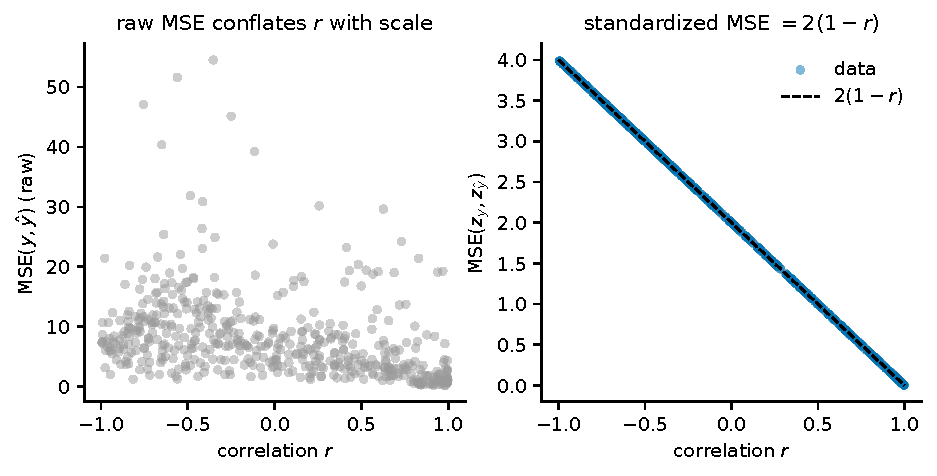
\includegraphics[width=\linewidth]{figures/fig1_geometry.pdf}
\caption{Geometry of the standardized-MSE / Pearson identity (Proposition~\ref{prop:1}).}
\label{fig:geometry}
\end{figure*}

\begin{figure*}[tbp]
\renewcommand{\familydefault}{\sfdefault}\normalfont
\centering
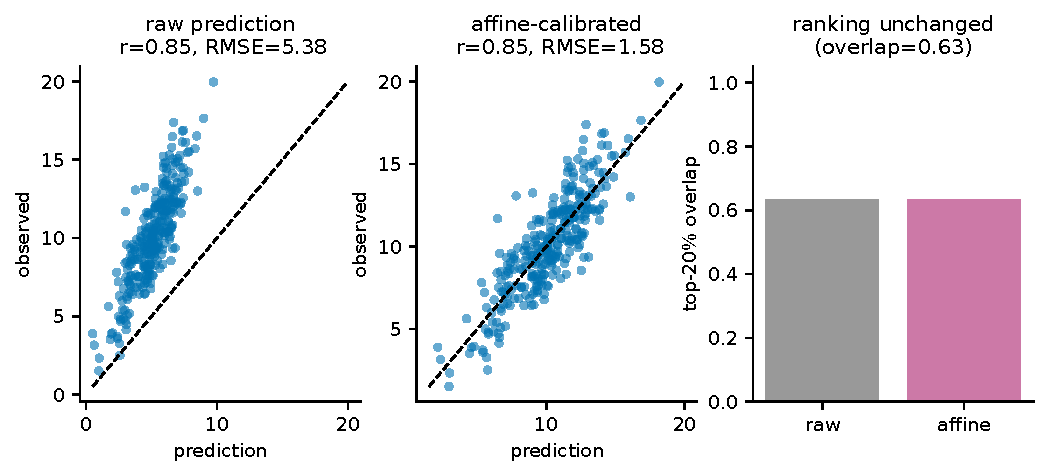
\includegraphics[width=\linewidth]{figures/fig2_simulation.pdf}
\caption{Controlled simulation of Proposition~\ref{prop:2}: a well-correlated but
mis-scaled prediction (left) is corrected by affine calibration (middle) ---
RMSE falls while Pearson $r$ is unchanged --- and the top-$20\%$ selection
overlap is identical before and after (right).}
\label{fig:simulation}
\end{figure*}

\begin{figure*}[tbp]
\renewcommand{\familydefault}{\sfdefault}\normalfont
\centering
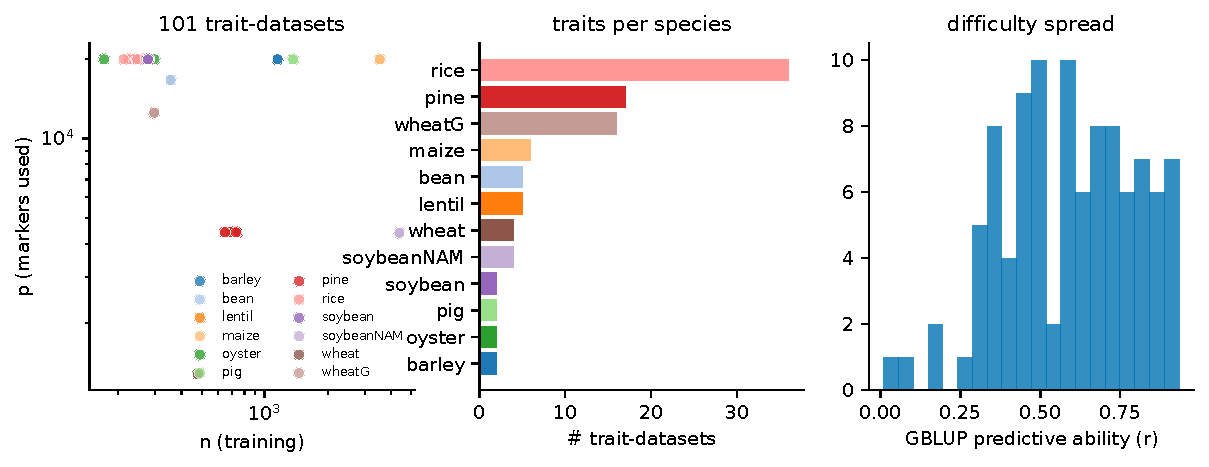
\includegraphics[width=\linewidth]{figures/fig3_datasets.pdf}
\caption{Dataset map: size, dimensionality and predictability across species.}
\label{fig:datasets}
\end{figure*}

\begin{figure*}[tbp]
\renewcommand{\familydefault}{\sfdefault}\normalfont
\centering
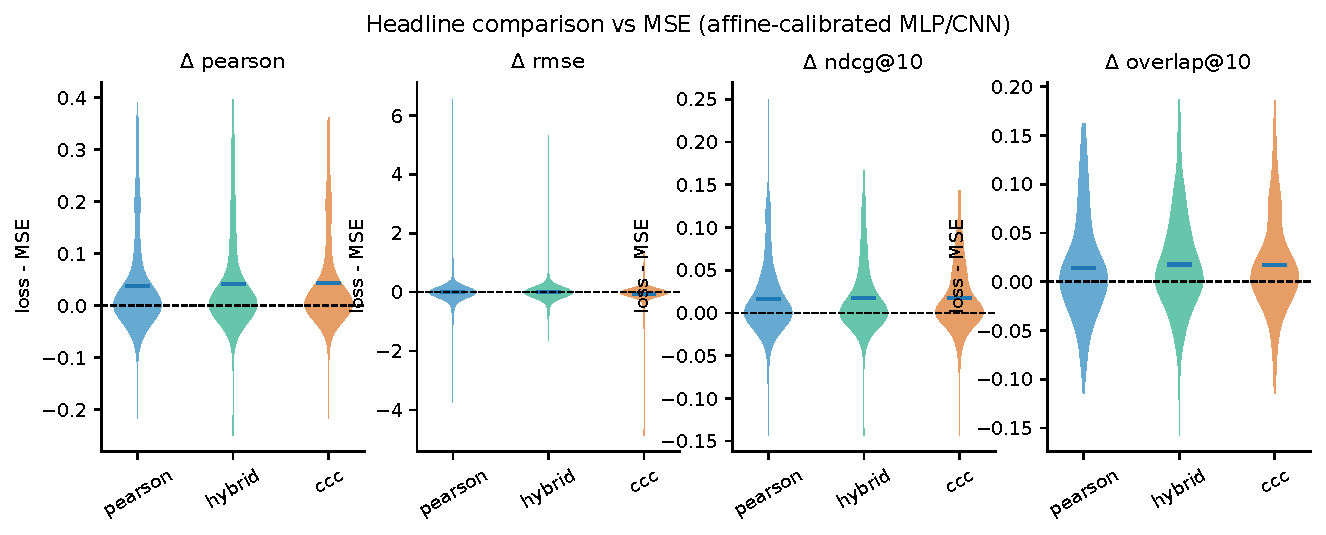
\includegraphics[width=\linewidth]{figures/fig4_loss_comparison.pdf}
\caption{Loss comparison: $\Delta$ versus MSE for Pearson, hybrid and CCC losses.}
\label{fig:loss}
\end{figure*}

\begin{figure*}[tbp]
\renewcommand{\familydefault}{\sfdefault}\normalfont
\centering
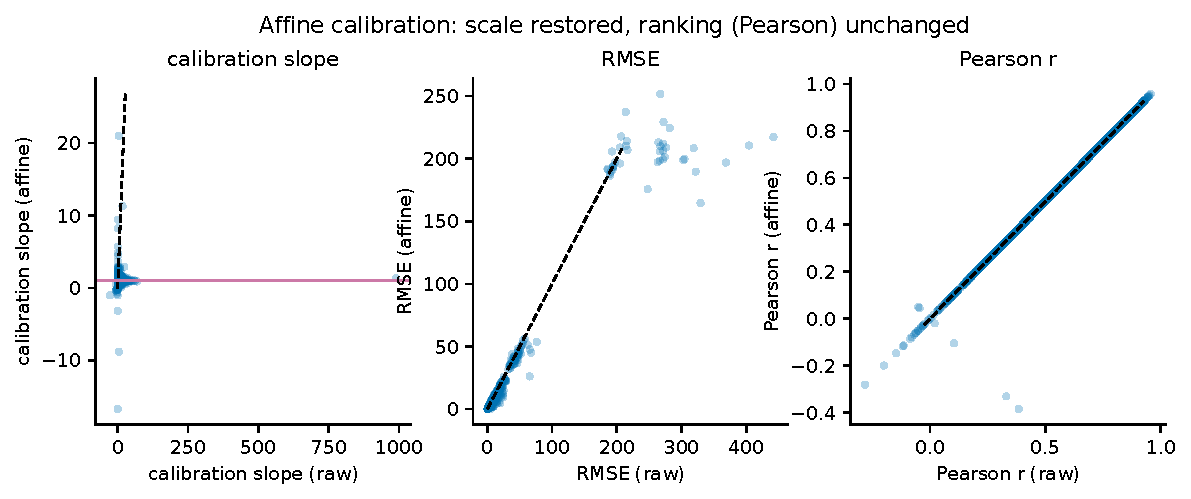
\includegraphics[width=\linewidth]{figures/fig5_calibration.pdf}
\caption{Affine calibration restores scale and offset while leaving Pearson unchanged.}
\label{fig:calibration}
\end{figure*}

\begin{figure*}[tbp]
\renewcommand{\familydefault}{\sfdefault}\normalfont
\centering
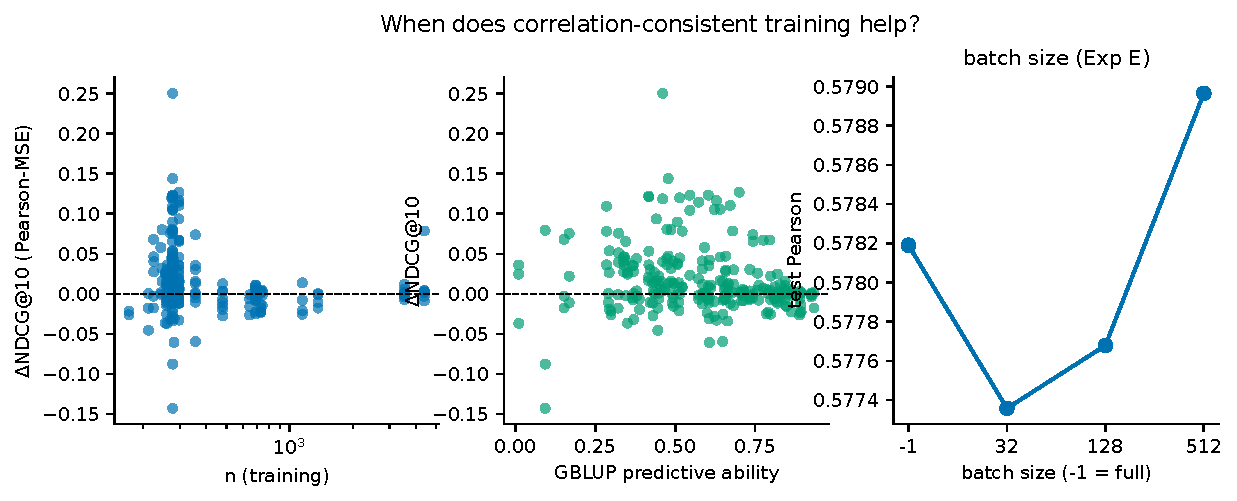
\includegraphics[width=\linewidth]{figures/fig6_meta.pdf}
\caption{When does correlation-consistent training help?}
\label{fig:meta}
\end{figure*}

% Full-width table (spans both columns)
\begin{table*}[htbp]
\renewcommand{\familydefault}{\sfdefault}\normalfont
\centering
\caption{\bf The 101 trait--dataset combinations across 12 panels/sources (10 species;
10 panels from EasyGeSe, plus CIMMYT wheat and SoyNAM). $n$ is the number of genotypes, $p$ the markers used
(after MAF filtering and the 20{,}000-marker variance cap), and GBLUP $r$ the mean
within-dataset predictive ability of GBLUP (a difficulty index).}
\label{tab:datasets}
\begin{tableminipage}{\textwidth}
\begin{tabularx}{\textwidth}{Xrrrrl}
\hline
\header Species & $n$ & $p$ & traits & GBLUP $r$ & source\\
\hline
rice & 352 & 20{,}000 & 36 & 0.46 & EasyGeSe \\
pine & 925 & 4{,}421 & 17 & 0.82 & EasyGeSe \\
wheatG & 371 & 12{,}546 & 16 & 0.59 & EasyGeSe \\
maize & 4421 & 20{,}000 & 6 & 0.83 & EasyGeSe \\
bean & 444 & 16{,}707 & 5 & 0.57 & EasyGeSe \\
lentil & 324 & 20{,}000 & 5 & 0.79 & EasyGeSe \\
soybeanNAM & 5487 & 4{,}401 & 4 & 0.71 & SoyNAM \\
wheat & 599 & 1{,}279 & 4 & 0.46 & BGLR/CIMMYT \\
barley & 1438 & 20{,}000 & 2 & 0.58 & EasyGeSe \\
oyster & 372 & 20{,}000 & 2 & 0.38 & EasyGeSe \\
pig & 1709 & 20{,}000 & 2 & 0.31 & EasyGeSe \\
soybean & 346 & 20{,}000 & 2 & 0.40 & EasyGeSe \\
\hline
\end{tabularx}

\vspace{2pt}
{\footnotesize\raggedright The count of 12 panels/sources (spanning 10 species)
treats related germplasm
sharing a common crop as distinct panels: wheatG (EasyGeSe) and wheat (CIMMYT) are
separate sources, as are soybean (EasyGeSe) and soybeanNAM (SoyNAM)
panels of the same species drawn from different sources.\par}
\end{tableminipage}
\end{table*}

\bibliography{refs}

\end{document}
